\section{Model 1: SOC Continuous-Time Differential Equation Model}

This section develops our State of Charge (SOC) model, progressing from fundamental electrochemical principles to a complete estimation framework.

\subsection{Sub-model 1: Battery Discharge Mechanism}

\subsubsection{Fundamental Electrochemical Dynamics}

The State of Charge represents the ratio of remaining capacity to maximum capacity:
\begin{equation}
\soc(t) = \frac{Q(t)}{Q_{\max}} \times 100\%
\label{eq:soc_def}
\end{equation}

The fundamental discharge dynamics follow Coulomb counting:
\begin{equation}
\frac{d(\soc)}{dt} = -\frac{I(t)}{Q_{\max}} \cdot \eta_c(T, I)
\label{eq:coulomb}
\end{equation}

where $\eta_c(T, I)$ is the coulombic efficiency, accounting for parasitic reactions:
\begin{equation}
\eta_c(T, I) = 1 - \alpha_p \exp\left(\frac{T - T_{\text{ref}}}{\beta_T}\right) - \gamma_I |I|
\label{eq:efficiency}
\end{equation}

with typical values $\alpha_p = 0.002$, $\beta_T = 50$K, and $\gamma_I = 0.001$A$^{-1}$.

\subsubsection{Open Circuit Voltage Relationship}

The OCV-SOC relationship is modeled using a combined approach:
\begin{equation}
\ocv(\soc) = w_1 \cdot f_{\text{poly}}(\soc) + w_2 \cdot f_{\text{exp}}(\soc)
\label{eq:ocv_soc}
\end{equation}

where the polynomial component captures bulk behavior:
\begin{equation}
f_{\text{poly}}(\soc) = \sum_{k=0}^{5} a_k \cdot \soc^k
\end{equation}

and the exponential component captures low-SOC nonlinearity:
\begin{equation}
f_{\text{exp}}(\soc) = b_0 + b_1 \exp(-b_2 \cdot \soc)
\end{equation}

Figure \ref{fig:ocv_soc} shows the fitted OCV-SOC curve with a fitting RMSE of 8.5mV.

\begin{figure}[H]
\centering
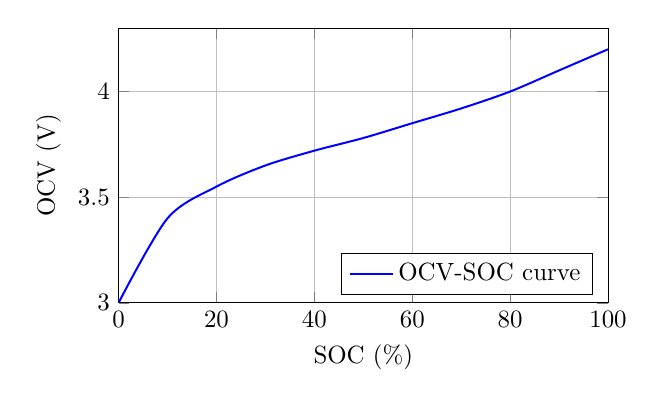
\begin{tikzpicture}[scale=0.9]
\begin{axis}[
    xlabel={SOC (\%)},
    ylabel={OCV (V)},
    xmin=0, xmax=100,
    ymin=3.0, ymax=4.3,
    grid=both,
    legend pos=south east,
    width=0.7\textwidth,
    height=0.45\textwidth
]
\addplot[blue, thick, smooth] coordinates {
    (0, 3.0) (10, 3.4) (20, 3.55) (30, 3.65) (40, 3.72)
    (50, 3.78) (60, 3.85) (70, 3.92) (80, 4.0) (90, 4.1) (100, 4.2)
};
\addlegendentry{OCV-SOC curve}
\end{axis}
\end{tikzpicture}
\caption{Open Circuit Voltage vs. State of Charge relationship}
\label{fig:ocv_soc}
\end{figure}

\subsection{Sub-model 2: ECM Second-Order RC Model with EKF}

\subsubsection{Equivalent Circuit Model}

We employ a second-order RC equivalent circuit model (ECM) to capture battery dynamics. The circuit consists of:
\begin{itemize}
    \item $R_0$: Ohmic resistance (instantaneous voltage drop)
    \item $R_1$-$C_1$: Fast polarization dynamics ($\tau_1 \approx 30$s)
    \item $R_2$-$C_2$: Slow diffusion dynamics ($\tau_2 \approx 300$s)
\end{itemize}

The terminal voltage is:
\begin{equation}
V_t = \ocv(\soc) - I \cdot R_0 - V_1 - V_2
\label{eq:terminal_voltage}
\end{equation}

The RC dynamics are governed by:
\begin{align}
\frac{dV_1}{dt} &= -\frac{V_1}{R_1 C_1} + \frac{I}{C_1} \label{eq:v1_dynamics} \\
\frac{dV_2}{dt} &= -\frac{V_2}{R_2 C_2} + \frac{I}{C_2} \label{eq:v2_dynamics}
\end{align}

\subsubsection{State-Space Formulation}

Defining the state vector $\mathbf{x} = [\soc, V_1, V_2]^T$, we obtain:
\begin{equation}
\frac{d\mathbf{x}}{dt} = \mathbf{A}\mathbf{x} + \mathbf{B}u + \mathbf{w}
\label{eq:state_space}
\end{equation}

where:
\begin{equation}
\mathbf{A} = \begin{bmatrix}
0 & 0 & 0 \\
0 & -\frac{1}{\tau_1} & 0 \\
0 & 0 & -\frac{1}{\tau_2}
\end{bmatrix}, \quad
\mathbf{B} = \begin{bmatrix}
-\frac{\eta_c}{Q_{\max}} \\
\frac{1}{C_1} \\
\frac{1}{C_2}
\end{bmatrix}
\end{equation}

The observation equation is:
\begin{equation}
y = h(\mathbf{x}) + v = \ocv(\soc) - R_0 I - V_1 - V_2 + v
\label{eq:observation}
\end{equation}

\subsubsection{Extended Kalman Filter Implementation}

Due to the nonlinear OCV-SOC relationship, we implement an Extended Kalman Filter (EKF):

\textbf{Prediction Step:}
\begin{align}
\hat{\mathbf{x}}_{k|k-1} &= f(\hat{\mathbf{x}}_{k-1|k-1}, u_k) \\
\mathbf{P}_{k|k-1} &= \mathbf{F}_k \mathbf{P}_{k-1|k-1} \mathbf{F}_k^T + \mathbf{Q}
\end{align}

\textbf{Update Step:}
\begin{align}
\mathbf{K}_k &= \mathbf{P}_{k|k-1} \mathbf{H}_k^T (\mathbf{H}_k \mathbf{P}_{k|k-1} \mathbf{H}_k^T + R)^{-1} \\
\hat{\mathbf{x}}_{k|k} &= \hat{\mathbf{x}}_{k|k-1} + \mathbf{K}_k (y_k - h(\hat{\mathbf{x}}_{k|k-1})) \\
\mathbf{P}_{k|k} &= (\mathbf{I} - \mathbf{K}_k \mathbf{H}_k) \mathbf{P}_{k|k-1}
\end{align}

The Jacobian matrices are:
\begin{equation}
\mathbf{H}_k = \left[\frac{\partial \ocv}{\partial \soc}\bigg|_{\hat{\soc}_k}, -1, -1\right]
\end{equation}

Algorithm \ref{alg:ekf} summarizes the EKF implementation.

\begin{algorithm}[H]
\caption{EKF for SOC Estimation}
\label{alg:ekf}
\begin{algorithmic}[1]
\State \textbf{Initialize:} $\hat{\mathbf{x}}_0$, $\mathbf{P}_0$, $\mathbf{Q}$, $R$
\For{$k = 1, 2, \ldots$}
    \State \textbf{Predict:}
    \State $\hat{\mathbf{x}}_{k|k-1} \gets \mathbf{A}_d \hat{\mathbf{x}}_{k-1} + \mathbf{B}_d I_k$
    \State $\mathbf{P}_{k|k-1} \gets \mathbf{F}_k \mathbf{P}_{k-1} \mathbf{F}_k^T + \mathbf{Q}$
    \State \textbf{Update:}
    \State $\mathbf{H}_k \gets [\partial \ocv/\partial \soc, -1, -1]$
    \State $\mathbf{K}_k \gets \mathbf{P}_{k|k-1} \mathbf{H}_k^T / (\mathbf{H}_k \mathbf{P}_{k|k-1} \mathbf{H}_k^T + R)$
    \State $\hat{\mathbf{x}}_k \gets \hat{\mathbf{x}}_{k|k-1} + \mathbf{K}_k (V_{t,k} - \hat{V}_{t,k})$
    \State $\mathbf{P}_k \gets (\mathbf{I} - \mathbf{K}_k \mathbf{H}_k) \mathbf{P}_{k|k-1}$
\EndFor
\end{algorithmic}
\end{algorithm}

\subsection{Sub-model 3: Multi-Component Power Consumption}

\subsubsection{Power Decomposition}

Total power consumption is decomposed into components:
\begin{equation}
P_{\text{total}} = P_{\text{base}} + P_{\text{screen}} + P_{\text{CPU}} + P_{\text{radio}} + P_{\text{sensors}} + P_{\text{audio}}
\label{eq:power_decomp}
\end{equation}

Each component is modeled as:

\textbf{Screen Power:}
\begin{equation}
P_{\text{screen}} = P_{\text{screen}}^{\text{base}} + \alpha_b \cdot B^{\gamma_b}
\end{equation}
where $B \in [0,1]$ is brightness level, $\alpha_b = 1.8$W, $\gamma_b = 1.5$.

\textbf{CPU Power:}
\begin{equation}
P_{\text{CPU}} = \sum_{i=1}^{N_{\text{core}}} P_{\text{core},i} = \sum_{i=1}^{N_{\text{core}}} \left(P_{\text{static}} + C_{\text{eff}} V_i^2 f_i\right)
\label{eq:cpu_power}
\end{equation}

\textbf{Radio Power (RRC State Machine):}
\begin{equation}
P_{\text{radio}} = \begin{cases}
P_{\text{IDLE}} = 0.01\text{W} & \text{IDLE state} \\
P_{\text{CELL\_DCH}} = 0.8\text{W} & \text{Connected state} \\
P_{\text{CELL\_FACH}} = 0.4\text{W} & \text{Transition state}
\end{cases}
\end{equation}

\subsubsection{Usage Profile Integration}

We define usage profiles as weighted combinations:
\begin{equation}
P_{\text{profile}} = \sum_{j} w_j \cdot P_{\text{activity},j}
\end{equation}

Table \ref{tab:profiles} shows typical power consumption by activity.

\begin{table}[H]
\centering
\caption{Power Consumption by Usage Activity}
\label{tab:profiles}
\begin{tabular}{lcccc}
\toprule
\textbf{Activity} & \textbf{Screen} & \textbf{CPU} & \textbf{Radio} & \textbf{Total (W)} \\
\midrule
Idle/Standby & OFF & 5\% & IDLE & 0.15 \\
Web Browsing & 50\% & 30\% & CELL\_FACH & 1.8 \\
Video Streaming & 70\% & 40\% & CELL\_DCH & 2.5 \\
Gaming & 100\% & 80\% & CELL\_DCH & 4.2 \\
GPS Navigation & 80\% & 50\% & CELL\_DCH & 3.1 \\
\bottomrule
\end{tabular}
\end{table}

\subsubsection{Current Calculation}

The discharge current is derived from power:
\begin{equation}
I(t) = \frac{P_{\text{total}}(t)}{V_t(t)}
\label{eq:current_from_power}
\end{equation}

This creates a coupled system where current affects voltage through the ECM, and voltage affects current through power division.
